\documentclass{article}

\usepackage[T1]{fontenc}

\usepackage{fancyhdr}
\usepackage{extramarks}
\usepackage{amsmath}
\usepackage{amsthm}
\usepackage{amsfonts}
\usepackage{tikz}
\usepackage{algorithm}
\usepackage{algpseudocode}
\usepackage{enumitem}

\usepackage[mono=false]{libertine}


\usetikzlibrary{automata,positioning}

%
% Basic Document Settings
%

\topmargin=-0.45in
\evensidemargin=0in
\oddsidemargin=0in
\textwidth=6.5in
\textheight=9.0in
\headsep=0.25in

\linespread{1.1}

\pagestyle{fancy}
\lhead{\hmwkAuthorName}
\chead{\hmwkClass \hmwkSection}
\rhead{\hmwkTitle}
\lfoot{\lastxmark}
\cfoot{\thepage}

\renewcommand\headrulewidth{0.4pt}
\renewcommand\footrulewidth{0.4pt}

\setlength\parindent{0pt}

%
% Create Problem Sections
%

\newcommand\tab[1][1cm]{\hspace*{#1}}

\newcommand{\enterProblemHeader}[1]{
    \nobreak\extramarks{}{Problem \arabic{#1} continued on next page\ldots}\nobreak{}
    \nobreak\extramarks{Problem \arabic{#1} (continued)}{Problem \arabic{#1} continued on next page\ldots}\nobreak{}
}

\newcommand{\exitProblemHeader}[1]{
    \nobreak\extramarks{Problem \arabic{#1} (continued)}{Problem \arabic{#1} continued on next page\ldots}\nobreak{}
    \stepcounter{#1}
    \nobreak\extramarks{Problem \arabic{#1}}{}\nobreak{}
}

\setcounter{secnumdepth}{0}
\newcounter{partCounter}
\newcounter{homeworkProblemCounter}
\setcounter{homeworkProblemCounter}{1}
\nobreak\extramarks{Problem \arabic{homeworkProblemCounter}}{}\nobreak{}

%
% Homework Problem Environment
%
% This environment takes an optional argument. When given, it will adjust the
% problem counter. This is useful for when the problems given for your
% assignment aren't sequential. See the last 3 problems of this template for an
% example.
%
\newenvironment{homeworkProblem}[1][-1]{
    \ifnum#1>0
        \setcounter{homeworkProblemCounter}{#1}
    \fi
    \section{Problem \arabic{homeworkProblemCounter}}
    \setcounter{partCounter}{1}
    \enterProblemHeader{homeworkProblemCounter}
}{
    \exitProblemHeader{homeworkProblemCounter}
}

%
% Homework Details
%   - Title
%   - Due date
%   - Class
%   - Section/Time
%   - Instructor
%   - Author
%

\newcommand{\hmwkTitle}{Homework\ \#6}
\newcommand{\hmwkDueDate}{April 24, 2018}
\newcommand{\hmwkClass}{Design and Analysis of Algorithms}
\newcommand{\hmwkClassInstructor}{Professor Kasturi Varadarajan}
\newcommand{\hmwkSection}{ (CS:5350)}
\newcommand{\hmwkAuthorName}{\textbf{Heather Kemp}}

%
% Title Page
%

\title{
    \vspace{2in}
    \textmd{\textbf{\hmwkClass:\ \hmwkTitle}}\\
    \normalsize\vspace{0.1in}\small{Due\ in\ class,\ at\ 9:30am,\ on\ \hmwkDueDate}\\
    \vspace{0.1in}\large{\textit{\hmwkClassInstructor}}
    \vspace{3in}
}

\author{\hmwkAuthorName}
\date{}

\renewcommand{\part}[1]{\textbf{\large Part \Alph{partCounter}}\stepcounter{partCounter}\\}

%
% Various Helper Commands
%

% Useful for algorithms
\newcommand{\alg}[1]{\textsc{\bfseries \footnotesize #1}}

% For derivatives
\newcommand{\deriv}[1]{\frac{\mathrm{d}}{\mathrm{d}x} (#1)}

% For partial derivatives
\newcommand{\pderiv}[2]{\frac{\partial}{\partial #1} (#2)}

% Integral dx
\newcommand{\dx}{\mathrm{d}x}

% Alias for the Solution section header
\newcommand{\solution}{\textbf{\large Solution}}

% Probability commands: Expectation, Variance, Covariance, Bias
\newcommand{\E}{\mathrm{E}}
\newcommand{\Var}{\mathrm{Var}}
\newcommand{\Cov}{\mathrm{Cov}}
\newcommand{\Bias}{\mathrm{Bias}}

% Set from 1 to N
\newcommand{\XYZ}[1]{\left\{1,\ldots,{#1}\right\}}
\newcommand{\Break}{\textbf{break} }

\begin{document}

\maketitle

\pagebreak

\begin{homeworkProblem}

For any flow network $G$ and any vertices $u$ and $v$ let \alg{bottleneck}$_G(u,v)$ denote the maximum, over all paths $\pi$ in $G$ from $u$ to $v$, of the minimum-capacity edge along $\pi$.

\begin{enumerate}[label=\alph*]
\item ) Describe and analyze an algorithm to compute \alg{bottleneck}$_G(s,t)$ in $O(E$log$V)$ time. 
\end{enumerate}

\solution\\

\part 

Based on the definition of bottlenecks from the reading, this problem is interpreted to mean to return the value of the greatest bottleneck value in the flow network $G$. If the desired return was vertex or edge that produces the maximum bottleneck, this algorithm can trivially be modified at lines 28-35 to not only retain the minimumWeight, but also the vertex or edge associated with that minimumWeight, and then return that minimum edge or vertex instead of minimum weight at the end.

\begin{algorithm}
	\begin{algorithmic}[1]
		\State{G $\gets$ desired flow network}
		\Function{BottleNeck$_{G}$}{$s, t$}
		
		\State{$heap \gets$ new binary heap}
		\For{vertex $currentVertex$ in $G.vertices$}
			\If{$currentVertex === s$}
				\State{$currentVertex.weight \gets \infty$}
			\Else
				\State{$currentVertex.weight \gets -\infty$}
			\EndIf
			\State{$heap$.add($currentVertex$)}
		\EndFor
		
		\State{$currentVertex \gets s$}
		
		\While{$t.visited == false$}
			\State{$currentVertex.visited \gets true$}
			\For{vertex $neighbor$ in $currentVertex.neighbors$}
				\If{$neighbor.visited == false$}
					\State{$currentEdge \gets$ edge between $currentVertex$ and $neighbor$}
					\If{$currentEdge.weight > neighbor.weight$}
						\State{$heap.$remove$(neighbor)$}
						\State{$neighbor.predecessor \gets currentVertex$}
						\State{$neighbor.weight \gets currentEdge.weight$}
						\State{$heap.$add($neighbor$)}
					\EndIf
				\EndIf
			\EndFor
			\State{$currentVertex \gets heap.$removeMax()}
		\EndWhile
		
		\State{$minimumWeight \gets \infty$}
		\State{$currentVertex \gets t$}
		\While{$currentVertex != s$}
			\State{$currentEdge \gets$ edge between $currentVertex$ and $currentVertex.predecessor$}
			\State{$minimumWeight \gets$ minimum($currentEdge.weight, minimumWeight$)}
			\State{$currentVertex \gets currentVertex.predecessor$}
		\EndWhile
		\State{\Return $minimumWeight$}
		\EndFunction
	\end{algorithmic}
\end{algorithm}

This algorithm was based off of the optimized Prim's algorithm using a binary heap. It is broken up into approximately three different pieces: Lines 4-11, Lines 12-27, and Lines 28-35, which will henceforth be referred to as the first, second, and third sections respectively. \\

(Algorithm on Next Page) \\

In the first section, we create our new binary heap to keep track of our vertices' weights. We use a binary heap due to its ability to obtain the max value in $O(1)$ time, and insert and remove values in $O(log(n))$ time, which is what allows us to optimize our algorithm. To properly set up the binary heap, we set all of our vertices to have a weight of $-\infty$, excluding our source vertex, $s$, which we set to $\infty$ to guarantee that we start with it in section 2, where we will be removing the max value, as we want our path to be guaranteed to start with the source. This is done in $O(v*log(v))$ time based on the definition of a binary heap as stated above. \\

In the second section, we start with s, and then visit all of the neighbors of our current vertex. We only need to review the vertex if we haven't visited it before. We define visiting as having checked all of the neighbors' edges, so we only mark the current node as visited, not its neighbors as we cycle through them, as we don't check their edges yet. In our visiting of the edge between the neighbors and our current node, we only update its weight if it is greater than the edge between the current vertex and its neighbors, as we are looking to find the maximum minimum cut, and wish to obtain the greatest value. We also link the predecessor to the current vertex to, again, be able to traverse up the path we made after we finish reaching t. For the section of Lines 18 - 22, as a binary heap takes log(n) time to remove and add values, the overall runtime is $O(log(v))$. As we only execute this when the neighbor is not visited, though, that means that the max we call this segment is twice per edge, making the resulting runtime for this segment $O(E*log(v) + V*log(v))$, or $O(E*log(v)),$ as we know that there is guaranteed to be a greater than or equal to number of edges relative to the vertices, as there must be at least one edge per vertex for it to be a connected graph as the problem states. Removing the max value is, as by the definition of a binary heap, is $O(1)$, so the entire section is $O(E*log(v))$. \\

In the third section, we traverse from $t$ to $s$ using this maximum path that we've found. We simply keep track of what the minimum is during this search, using our predecessor nodes which we set in the second section to travel back to $s$, which we are guaranteed to reach as we started our maximum tree with it, and return the minimum weight at the end. In the worst case of all of the vertices being connected in a line-like structure, this would be $O(v)$, as our comparisons are constant. \\

Thus, our three sections have a runtime of $O(v*log(v)), O(E*log(v)),$ and $O(v)$. As discussed in the analysis of the second section, $v*log(v)$ is less than $E*log(v)$ for runtime, and thus, the overall runtime is $O(E*log(v))$.

\end{homeworkProblem}

\pagebreak

\begin{homeworkProblem}

Suppose you have already computed a maximum flow $f*$ in a flow network $G$ with \emph{\color{red}{integer}} edge capacities.

\begin{enumerate}[label=\alph*]
\item ) Describe and analyze an algorithm to update the maximum flow after the capacity of a single edge is increased by 1.
\item ) Describe and analyze an algorithm to update the maximum flow after the capacity of a single edge is decreased by 1.
\end{enumerate}

Both algorithms should be significantly faster than recomputing the maximum flow from scratch. \\

\solution\\

\part 

\begin{algorithm}
	\begin{algorithmic}[1]
		\Function{MaxFlowIncrement}{$G, s, t$} \Comment{$G$ is assumed to have $f*$ stored as a variable, and be already updated as it wishes to be}
		
		\State{$BFSPath \gets BFS(G, s, t)$} \Comment{Returns the edges that make up the BFS path, as defined in the original algorithm}
		\If{$BFSPath != null$} \Comment{We can assume it probably will be if we have f*, but just to be sure}
			\State{$minimumResidualCapacity \gets \infty$}
			\For{Edge $e$ in $BFSPath$}
				\If{Residual Capacity of $e < minimumResidualCapacity$}
					\State{$minimumResidualCapacity \gets$ Residual Capacity of $e$}
				\EndIf
			\EndFor
			\For{Edge $e$ in $BFSPath$}	
				\If{$e$ is a forward edge}
					\State{$G.f*[e] \gets G.f*[e] + minimumResidualCapacity$}
				\Else \Comment{Is a backward edge}
					\State{$G.f*[e] \gets G.f*[e] - minimumResidualCapacity$}
				\EndIf
			\EndFor
			\State{\Return $G.f*$}
		\EndIf
		\EndFunction
	\end{algorithmic}
\end{algorithm}

This algorithm is based off of the original Ford-Fulkerson algorithm, but altered so that it starts with a prior maximum flow already calculated. Essentially, as we are only incrementing a value by one, we can just pick up where we left off, and treat the execution of this algorithm as the last part of the while loop in the original algorithm. This algorithm only works because we can operate on the assumption that the maximum flow was already calculated for us, and that we can only update the graph edges by 1. As such, as the only thing that changed between the original algorithm and this new one is the lack of a while loop, as, again, we are just 'continuing' the previous iterations, the rest of the algorithm is assumed to be intuitive from Jeff's notes.\\

As stated by Jeff's notes, performing a breadth/depth-first search to find an augmenting path will take $O(V + E)$ time, and as this, along with traversing those edges separately, is all that we do in this algorithm, we can conclude that this algorithm runs in $O(V + E)$ time, or just $O(E)$, as E is bounded by $V^2$. This makes sense, as, again, according to Jeff's notes, the original Ford-Fulkerson algorithm, which starts from having no maximum flow calculated, runs in $O(E|f*|)$ time, where $f*$ is the actual maximum flow. As we start with a maximum flow, and only increment by 1, we only do 1 iteration, which makes our run time $O(E*1)$, or just $O(E)$.
		
\part 

\begin{algorithm}
	\begin{algorithmic}[1]
		\Function{MaxFlowDecrement}{$G, s, t,$} \Comment{$G$ is assumed to have $f*$ stored as a variable, and be already updated as it wishes to be}
		\State{$changedEdge \gets null$}
		\For{Edge $currentEdge$ in $G.edges$}
			\If{$currentEdge.capacity - currentEdge.flow < 0$}
				\State{$changedEdge \gets currentEdge$}
			\EndIf
		\EndFor
		\If{$changedEdge == null$} \Comment{The max flow hasn't been affected}
			\State{\Return $G.f*$}
		\EndIf
		\State{$BFSPath \gets BFSWith(G, s, t, changedEdge)$} \Comment{A trivial update to the original BFS algorithm to make sure the returned path contains $changedEdge$}
		\If{$BFSPath != null$} \Comment{We can assume it will exist, but just to make sure}
			\For{Edge $e$ in $BFSPath$}	
				\State{$G.f*[e] \gets G.f*[e] - 1$}
			\EndFor
		\EndIf
		\State{$BFSPath \gets BFS(G, s, t)$} \Comment{Returns the edges that make up the BFS path, as defined in the original algorithm}
		\If{$BFSPath != null$} \Comment{We can assume it probably will be if we have $f*$, but just to be sure}
			\State{$minimumResidualCapacity \gets \infty$}
			\For{Edge $e$ in $BFSPath$}
				\If{Residual Capacity of $e < minimumResidualCapacity$}
					\State{$minimumResidualCapacity \gets$ Residual Capacity of $e$}
				\EndIf
			\EndFor
			\For{Edge $e$ in $BFSPath$}	
				\If{$e$ is a forward edge}
					\State{$G.f*[e] \gets G.f*[e] - minimumResidualCapacity$}
				\Else \Comment{Is a backward edge}
					\State{$G.f*[e] \gets G.f*[e] + minimumResidualCapacity$}
				\EndIf
			\EndFor
			\State{\Return $G.f*$}
		\EndIf
		\EndFunction
	\end{algorithmic}
\end{algorithm}

The way this algorithm works, like the previous problem, is quite simple, as we start off with our previous $f*$. As not all reductions in the flow will change the max flow (for example, 4/10 changing to 4/9 will not change our result), and so we only proceed with the rest of the algorithm if there is now a negative residual capacity (which might require recalculation). Then we start off by finding a path from our source, $s$, to our sink, $t$, along our flow that contains the decremented edge. This is trivially done by a anything-first-search, which can be done in $O(V + E)$ time, or just $O(E)$, as explained in the previous problem. We then traverse through all of these edges, subtracting 1 from the flow for each edge in the path in order to satisfy having decremented our edge. We can do this as by assuming there is no backwards edges in our calculated path, which seems to be a reasonable assumption, as we could repeat the selection until we have no back edges, which is expected to be only a few times. This is an $O(E)$ operation, as we visit each edge once in the worst case. This is the only thing that differs between part A and this solution, as now, we run into the possibility of our new flow being suboptimal, as we decreased its max flow. However, as we only decremented it by one, we know that it is at most only 1 less than the optimal flow, and so only one iteration of Ford-Fulkerson will suffice. As stated before, we can pick up where we 'left off', and continue the Ford-Fulkerson algorithm as if this were the last iteration, which is an $O(E)$ operation. Overall, this algorithm, as a result, performs as $O(E)$.

\end{homeworkProblem}

\pagebreak

\begin{homeworkProblem}

$\tab$ The Island of Sodor is home to a large number of towns and villages, connected by an extensive rail network. Recently, several cases of a deadly contagious disease (either swine flu or zombies; reports are unclear) have been reported in the village of Ffarquhar. The controller of the Sodor railway plans to close down certain railway stations to prevent the disease from spreading to Tidmouth, his home town. No trains can pass through a closed station. To minimize expense (and public notice), he wants to close down as few station as possible. However, he cannot close the Ffarquhar station, because that would expose him to the disease, and he cannot close the Tidmouth station, because then he couldn't visit his favorite pub.

\tab Describe and analyze an algorithm to find the minimum number of stations that must be closed to block all rail travel from Ffarquhar to Tidmouth. The Sodor rail network is represented by an undirected graph, with a vertex for each station and an edge for each rail connection between two stations. Two special vertices $f$ and $t$ represent the stations in Ffarquhar and Tidmouth.

\tab For example, given the following input graph, your algorithm should return the number 2.

\begin{figure}[h]
	\centering
		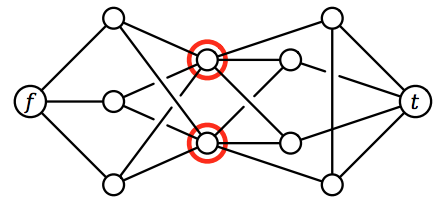
\includegraphics[scale=.75]{images/problem3}
\end{figure}

\solution\\

\begin{algorithm}
	\begin{algorithmic}[1]
		\Function{SodorMinClosures}{$G, f, t$} 
		\State{$newGraph \gets$ new graph with just $f$ and $t$ inserted}
		\For{Vertex $currentVertex$ in $G.vertices$}
			\If{$currentVertex != f$ AND $currentVertex != t$}
				\State{$vertex_f, vertex_c \gets$ new Vertex} \Comment{$currentVertex$'s flow and capacity}
				\State{$vertex_f.$addEdge($vertex_c, \infty$)} \Comment{$addEdge(vertex, weight)$: adds edge to $vertex$ with $weight$ weight}
				\State{$newGraph$.insert($vertex_f, vertex_c$)}
				\State{Link reference of $vertex_f$ and $vertex_c$ in $newGraph$ to $currentVertex$} 
			\EndIf
		\EndFor
		\For{Vertex $currentVertex$ in $G.vertices$}
			\If{$currentVertex != f$ OR $currentVertex != t$}
				\For{Vertex $neighbor$ in $currentVertex.neighbors$}
					\If{$currentVertex != f$}
						\State{$neighbor.c.$addEdge($currentVertex.f, $1)}
					\EndIf
					\If{$currentVertex != t$}
						\State{$currentVertex.c$.addEdge($neighbor.f,$ 1)}
					\EndIf
				\EndFor
			\EndIf
		\EndFor
		\State{\Return minimumCut($newGraph$)}

		\EndFunction
	\end{algorithmic}
\end{algorithm}

This problem is very similar to the minimum-cut algorithm, but instead of using edges, we would ideally like to use vertices. However, that would involve us re-inventing the wheel by recreating this algorithm entirely, and so, we are going to edit our input graph to make a suitable graph. We will construct a graph with the edges we want for set up as un-prioritized and those we can to consider for removal as prioritized. We assume that we can construct a min-cut algorithm which priorities the high-capacity edges for removal, meaning edges we set to $\infty$ will be removed more likely than ones that are assigned to 1.\\

The first step that we do is similar to the Ford-Fulkerson proof from Jeff's notes which breaks up two connected nodes into three connected nodes. In our case, though we will be looking to make a flow and a capacity vertex in our graph for nodes outside of our desired $s$ and $t$, as we don't want to consider these for removal. We then add edges based on the original graph, so that if $x$ and $y$ are connected, then $x.c$ and $y.f$ are connected and $y.c$ and $x.f$ are connected. As we aren't deleting edges, and all of the original nodes are still connected through their new $c$ and $f$ vertices, we know that we did not remove any possible paths or flows from the original graph. This is, again, a similar proof step to the Ford-Fulkerson proof. The runtime of this part of the program is trivial to compute, as inserting an edge and vertex is $O(1)$, and, as we split $V - 2$ vertices, including their edges, into 2, we see we have $2V + 2E$, which simplifies to $O(E)$, using logic similar to the previous problem on how $V + E$ simplifies to $E$.\\

Having proved this allows us to apply our minimum-cut algorithm. Take note that we assigned the 'inner' edges, or the ones between the capacity and the flow of the vertices, to be $\infty$, or to be more likely to be removed, because once we remove these cuts, we've 'removed' it from the graph, as our flow can no longer pass through this node. While the nodes remain, since they prevent the node from actually being used in the path calculation, we do not need to remove the actual nodes. The minimum cut was analyzed by Jeff in his notes to be $O(VE)$ by the Maxflow Mincut theorem, and, as a result, as we are just using this same algorithm, we can generalize this step to have that runtime. \\

The runtime of both of these sections is $O(E)$ and $O(VE)$ respectively, which, through basic arithmetic, is seen to be bounded by $O(VE)$.

\end{homeworkProblem}

\pagebreak

\begin{homeworkProblem}

Suppose we are given an $n$ x $n$ square grid, some of whose squares are colored black and the rest white. Describe and analyze an algorithm to determine whether tokens can be placed on the grid so that

\begin{enumerate}
\item every token is on a white square;
\item every row of the grid contains exactly one token; and
\item every column of the grid contains exactly one token
\end{enumerate}

\begin{figure}[h]
	\centering
		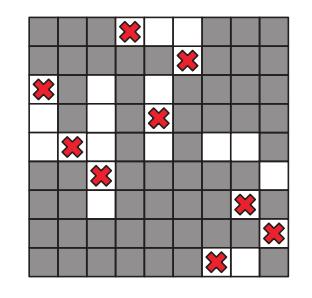
\includegraphics[scale=.75]{images/problem4}
\end{figure}

Your input is a two dimensional array $IsWhite$[1..$n$, 1..$n$] of booleans, indicated which squares are white. Your output is a single boolean. For example, given the grid above as input, your algorithm should return \alg{True}. \\

\solution\\

As this problem and the subsequent one take place in the graph/flow application, it is assumed that, for each of these problems, a graph must somehow be constructed, and then a max flow or min cut must be applied to the new graphs.\\

[Algorithm on next page] \\

\begin{algorithm}
	\begin{algorithmic}[1]
		\Function{BWTokenChecker}{$isWhite[1...n, 1...n]$} 
		\State{$board \gets$ new graph}
		\State{$start, end \gets$ new vertex} \Comment{Row 0 and Row $n$+1: bounds}
		\State{$board$.insert($start$); $board$.insert($end$)}
		\For{int $i \gets$ 1; $i <= n$; $i++$}
			\State{$rowVertex, columnVertex \gets$ new vertex}
			\State{$board$.insert($rowVertex$); $board$.insert($columnVertex$)}
			\State{$start$.addEdge($rowVertex,$ 1)}
			\State{$columnVertex$.addEdge($end$,1)}]
		\EndFor
		\For{int $currentRow \gets$ 1; $currentRow <= n$; $currentRow++$}
			\For{int $currentColumn \gets$ 1; $currentColumn <= n$; $currentColumn ++$}
				\If{$isWhite[currentRow, currentColumn] == $true}
					\State{$newWhiteTile \gets$ new vertex}
					\State{$board.$insert($newWhiteTile$)}
					\State{$currentRowVertex \gets rowVertex$ for $currentRow$}
					\State{$currentColumnVertex \gets columnVertex$ for $currentColumn$}
					\State{$currentRowVertex$.addEdge($newWhiteTile$)}
					\State{$newWhiteTile$.addEdge($currentColumnVertex$)}
				\EndIf
			\EndFor
		\EndFor
		\State{\Return maxFlow($board$).flow == $n$}
		
		\EndFunction
	\end{algorithmic}
\end{algorithm}

As stated prior to the problem, our first step is going to be attempting to transform our board into a graph. We begin by constructing start and end nodes, which we use to, of course, give us a start and end, for any algorithm we choose. That is, start and end can function as our source and our sink. This is, of course, an $O(1)$ operation, as we're just adding vertices to our graph.  \\

The next section, a for loop, creates $n$ row and column nodes, which connect to $start$ and $end$ respectively. We do this to bound our flow to meet the requirement of having one token per row and column. As there are $n$ edges going out of start and only $n$ edges going into end, with only a capacity of 1, we have limited our flow to be $n$ in both cases. That is, if each column and each row has at least one white tile to be able to place its piece, then we know we can place our pieces properly in the columns or rows, and when both of these conditions are met, which is during a max flow of $n$, assuming we only visit white tiles, then we can return true. This, of course, plays a role in our assignment during the next step. For the runtime of this segment, though, we should see it is intuitively $O(n)$, as inserting a vertex and edge is $O(1)$ and we do this $n$ times. \\

The interesting part of the algorithm comes in the next section, the nested for loops. This section, as stated prior, is addressing the third condition, which is making sure pieces can only be placed on white tiles. To address this, we simply only add inner vertices to our board if we know the tile is white from $isWhite$. When we do add them to our board, we keep up with the connection flows we made in the previous section to allow our conditions to remain true. That is, as we connect start to the rows and the columns to the end, we also are going to assign the row to the tile and the tile to the column. This part is, again, intuitively $O(n^2)$, as we loop through all of the tiles to check their status, and even if all of the tiles are white, all of our operations are $O(1)$. \\

Thus, as we just covered, all of our conditions are met, provided that we have a max flow of $n$, as stated why in the second section. We can assume we are utilizing the $O(VE)$ runtime max flow algorithm that was described in Jeff's notes. Our vertices are 2 nodes for the start and end, $2n$ nodes ($n$ nodes for the rows, $n$ nodes for the columns) and the possibility of $n^2$ nodes if the board is all white tiles. Our edges are $2n$ ($n$ edges for the start to rows and $n$ edges for the columns to end) and the possibility of $2n^2$ edges, as, as seen in our algorithm, we add two edges for each white tile, which, as we just established, is at worst $n^2$. Thus, $O((2 + 2n + n^2)(2n + n^2))$, which is intuitively, when factored, bounded by $O(n^4)$. \\

Our overall algorithm is bounded by its parts, which are $O(1), O(n), O(n^2),$ and $O(n^4)$, which can be simplified into just being bounded by $O(n^4)$.

\end{homeworkProblem}

\pagebreak

\begin{homeworkProblem}

\tab $Ad-hoc$ networks are made up of low-powered wireless devices. In principle, these networks can be used on battlefields, in regions that have recently suffered from natural disasters, and in other hard-to-reach areas. The idea is that a large collection of cheap, simple devices could be distributed through the area of interest (for example, by dropping them from an airplane); the devices would then automatically configure themselves into a functioning wireless network.

\tab These devices can communicate only within a limited range. We assume all the devices
are identical; there is a distance $D$ such that two devices can communicate if and only if
the distance between them is at most $D$.

\tab We would like our ad-hoc network to be reliable, but because the devices are cheap
and low-powered, they frequently fail. If a device detects that it is likely to fail, it should
transmit its information to some other $backup$ device within its communication range. We
require each device $x$ to have $k$ potential backup devices, all within distance $D$ of $x$; we call
these $k$ devices the \textbf{\textit{backup set}} of x. Also, we do not want any device to be in the backup
set of too many other devices; otherwise, a single failure might affect a large fraction of
the network. 

\tab So suppose we are given the communication radius $D$, parameters $b$ and $k$, and an
array $d$[1 .. $n$, 1 .. $n$] of distances, where $d[i, j]$ is the distance between device $i$ and device
$j$. Describe an algorithm that either computes a backup set of size $k$ for each of the $n$
devices, such that no device appears in more than $b$ backup sets, or reports (correctly) that
no good collection of backup sets exists. \\

\solution\\

As stated in the previous problem solution introduction, we will be attempting to convert this problem into a graph based on the problem criteria.\\

[Algorithm on next page] \\

\begin{algorithm}
	\begin{algorithmic}[1]
		\Function{AdHocChecker}{$D, b, k, d[1...n, 1...n]$} 
		\State{$field \gets$ new graph}
		\State{$start, end \gets$ new vertex}
		\State{$field$.insert($start$); $field$.insert($end$)}
		\For{int $i \gets$ 1; $i <= n$; $i++$} \Comment{Create all device vertices}
			\State{$device_i, deviceBackup_i \gets$ new vertex}
			\State{$field$.insert($device_i$), $field$.insert($deviceBackup_i$);}
			\State{$start$.addEdge($device_i, k$)}
			\State{$deviceBackup_i.$addEdge$(end, b)$}
		\EndFor
		\For{int $i \gets$ 1; $i <= n$; $i++$}
			\For{int $j \gets$ j; $j <= n$; $j++$}
				\If{$D >= d[i, j]$ AND $i != j$}
					\State{$device \gets device_j$ for $j$} \Comment{As assigned last for loop}
					\State{$deviceBackup \gets deviceBackup_i$ for $i$}
					\State{$device$.addEdge($deviceBackup$, 1)}
				\EndIf
			\EndFor
		\EndFor
		
		\State{$f* \gets$ MaxFlow($field$)}
		\State{$devicePairings \gets$ empty ArrayList}
		\If{$f*.flow != nk$}
			\State{\Return $devicePairings$} \Comment{Print some error/message}
		\Else
			\For{int $currentDevice \gets$ 1; $currentDevice <= n$; $currentDevice++$}
				\State{$currentDevicePairings \gets$ empty ArrayList}
				\For{int $currentBackup \gets$ 1; $currentBackup <= n$; $currentBackup++$}
					\State{$device \gets device_currentDevice$ for $currentDevice$} 
					\State{$deviceBackup \gets deviceBackup_currentBackup$ for $currentBackup$}
					\If{$f*[device, deviceBackup].flow >$ 0} \Comment{Positive flow}
						\State{$currentDevicePairings$.add($currentBackup$)}
					\EndIf
				\EndFor
				\State{$devicePairings.$add($currentDevicePairings$)}
			\EndFor
			\State{\Return $devicePairings$}
		\EndIf

		\EndFunction
	\end{algorithmic}
\end{algorithm}

This algorithm is very similar in its steps to the previous problem, only with different criteria with which we have to work with to maintain our conditions. Our first step is the very same though -- we create an empty graph with a start and end node to allow traversal through the graph from start to end. As explained before, this is an $O(1)$ operation. \\

Our next step, the first for loop we see, is also fairly similar. In this loop, we create two vertices for each device we have. Unlike row and column, this time, we have one vertex for the device as a broadcasting device, and the other vertex for the device as a backup device for some other device. We still link our start to our broadcasting device vertices and our backups to the end in order to monitor conditions the conditions of "[each of the $n$ devices must have] a backup set of size $k$" and "no device appears in more than $b$ backup sets". As we limit our broadcasting device edge capacities to be $k$ and our backup device edge capacity to be $b$, we are caping our flow at these respective values by our own restricted bottleneck. The actual calculation of what this flow must be will be addressed in a later step. However, as we've restricted our flow and have devised a way to monitor these conditions by ensuring our flow is in these ranges, at this point, just as before, we can consider them met. This part of the algorithm is $O(n)$, as inserting devices/edges is $O(1)$ and we do this $n$ times. \\

In the third step, which is the nested for loop, we begin actually establishing backup connections. All backup devices must be "within distance $D$ of [the device]", and, rather intuitively, cannot be a backup of itself. If it were, sending the backup would not do anything to save the data from the device before it crashes, and thus, we will not consider the device to be available to be a backup of itself. If both of these conditions are met, we assign an edge between the device and the symbolic backup of its linked device, assigned to be 1 so that our flow can total up to $k$ or $b$ as described in the previous step. As we only establish these connections in the case that both of our backup criteria are met, however, we can thus prove that no backups will be outside of the range required. Thus, at this point, assuming we implement our flow check correctly, all of our validation requirements have been met. This step is, intuitively, $O(n^2)$, as we utilize two for loops of size $n$ and all of our internal operations are $O(1)$. \\

The fourth step is to calculate the max flow to check our device capacities, as described briefly in the second section. As stated there, as we already bottlenecked our backup capacity to be less than or equal to $b$, we do not need to take it into consideration with this calculation. It will be implicitly handled in the max flow calculation, should a working set exist. However, the more crucial of the criteria is the  "[each of the $n$ devices must have] a backup set of size $k$". As this is a firm restriction, as opposed to a less than or equal to relationship, we chose to enforce this at the time of MaxFlow, as without it, we have nothing to return. This is, of course, simplified to be $n*k$ as the max flow, as, similarly to the last problem, we have $n$ edges of capacity $k$, and if our criteria is met, all of them should be meeting their capacity. That is, all of the devices should have $k$ backups. If not, we can return early with an empty list, as such a set can't exist. \\

As stated in Jeff's notes, MaxFlow can be implemented in $O(VE)$, and so we choose to utilize this implementation. Looking back at our previous steps, we see that we have only inserted a start and end vertex and two vertices for each device, which leaves us with $2n + 2$ vertices. On the other hand, we add $2n$ edges, as we connect start to each device and end to each backup device, and, in the worst case where every device is the backup of every other device, a max bound of $n^2$ edges. Thus, the MaxFlow($field$) call is on the runtime of $O((2n + 2) n^2)$, which, when factored, is seen to be bounded by $O(n^3)$. \\

The last step, the second nested for loop, is simply to make the list of pairings for the return. We only include edges, or say a device is the backup of another, if there was positive flow in the max flow we just calculated. That is, if it was used in calculating the max flow, we know its backup status is held, and thus, we can add it to the list. It should be noted that, as stated before, $b$ is bottlenecked by our end edges, so we don't run the risk of having more than $b$ backups, as the max flow can't return more backups (capacity 1) than $b$. As each for loop is of $n$ cycles, and arrayList insertion is O(1), this part of the algorithm runs in $O(n^2)$. \\

Our algorithms entire runtime is bounded by the sum of its parts, which are $O(1), O(n), O(n^2), O(n^3)$ and $O(n^2)$, all of which intuitively are bounded by $O(n^3)$.

\end{homeworkProblem}

\end{document}